\documentclass{article}
\usepackage{amsfonts} % \mathbb
\usepackage[margin=0.5in]{geometry}
\usepackage[utf8]{inputenc}
\usepackage{graphicx}
\usepackage[backend=biber, style=apa]{biblatex}
\usepackage{amsmath}
\DeclareMathOperator{\sign}{sign}
\bibliography{bibli}

\title{Robust Digital Envelope Estimation Via Geometric Properties of a Arbitrary Signal}
\author{
  Carlos Tarjano
  \and 
  Valdecy Pereira
  }

\begin{document}

\maketitle

\begin{abstract} % 250 words

% estimate parameters from the signal itself
% broadband
% Dominant frequency as by-product
% we define several entities in the process, introducing a new measure of discrete curve curvature, hoping to consolidate the terminology in the area

  % background  
  Despite being an elusive concept, mathematically well defined only for artificially generated waves, the temporal amplitude envelope of a signal is essential for its complete characterization, being the primary information carrying medium in spoken voice and telecommunications, for example.
  intuitively, the temporal envelope can be understood as a smooth function on the same variable as the principal wave, or temporal fine structure, that modulates the signal, responsible for its outer shape. It is implied in this definition that the envelope is non periodic in general and is thus better addressed by specific techniques diverse from those used in the analysis of the periodic, rapidly changing wave it encompasses.
  % motivation
  Envelope detection techniques have applications in areas like health, sound classification and synthesis, seismology and speech recognition. Despite of that, a general approach to envelope detection of signals with rich spectral content seems to be lacking, and most methods involve manual intervention, like filter design, based on prior knowledge about the wave under investigation.
  % objective
  In this paper we propose a framework that uses intrinsic characteristics of a signal to estimate its envelope, eliminating the necessity of parameter tuning.
  % methods
  The approach here described draws inspiration from general and differential geometry to isolate the frontier of an arbitrary signal. The concepts of alpha-shapes, concave hulls, arc-length parametrization and discrete curve curvature are adapted. We also define a pulse in the context of a arbitrary digital signal as a means to reduce dimensionality and subsequently, the complexity of the algorithm.
  % results
  
  % implications

\end{abstract}

{\bf Keywords:} DSP, alpha-shapes, envelope detection

\section{Introduction} % 500 words
% Opener sentence
Despite being ubiquitous in digital signal processing, the literature about envelope detection is very fragmented \parencite{2017LyonsDigital}. Besides, most envelope detection techniques are designed to account for very specific settings, like pure sinusoids with moderate noise contents, in line with the most common usages of those algorithms with artificial signals in the context of analog telecommunications.
% Literature review | Brief Context of Prior Research
In many natural signals, however, the temporal amplitude envelope of a signal plays a prominent role in the characteristics exhibited: According to \textcite{2017QiRelative}, for example, the envelope is at least as important as the fine structure of the soundwave in the context of the intelligibility of mandarin tones. That is also the case for English \parencite{1995ShannonSpeech}, where even envelopes modulating mostly noise were still capable of conveying meaning. The envelope helps to convey emotion and identity to the human voice \parencite{2018ZhuContributions}, and envelope preserving characteristics of concert halls are associated with their pleasantness \parencite{2011LokkiEngaging}.

% enumerate some uses in diverse areas

Also, the envelope is shown to add complexity to the spectral representation of a wave \parencite{2019TarjanoNeuro}, and a accurate description of the envelope would be useful for a subsequent spectral analysis. In the context of sound synthesis, for example, one would be able to apply different methods for the recreation of the envelope, more in line with its smooth, slow varying and non periodic nature and an different approach to the periodic and relatively fast changes of the temporal fine structure.

% Cite current algorithms

% Restate Your Question as Something Not Known or Fully Understood by Prior Research
Thus, in this paper we formulate a general approach to envelope detection, examining the intrinsic characteristics of a generic, spectrally complex wave in order to avoid parameter tuning.
% State the Significance of Your Question
While the robustness of the proposed approach allows it to be used as a plug in replacement for many methods encountered in the literature, we feel that it would be particularly useful for sound synthesis.
% State Your Claim | Objective | Hypothesis
% brief outlook on the structure of the paper




\section{Methodology} % 1000 words

% Essential background information
We start by defining a pulse as a series of consecutive samples in a discrete wave with the same signal. More formally, let $ W[i] \in \mathbb{R} \forall i \in \mathbb{N}_0, i < n \in \mathbb{N}_0 $ be a real, discrete and finite signal indexed, without loss of generality, over a subset of the natural numbers. This definition relates closely to the concept of an array or vector in programming languages, and is used in the interest of simplicity. A pulse $ P[j], j \in \mathbb{N}_0 $ in $ W $ can then be defined as a sequence of samples indexed by $ i $ such that $ \sign(W[a-1]) \ne \sign(W[a]) = \sign(W[a+1]) = \dots = \sign(W[b-1]) = \sign(W[b]) \ne \sign(W[b+1]) \forall a \le i \le b | a,b \in \mathbb{N}_0 $; that is to say, a cluster of samples between the change of sign. For a continuous function, that would correspond to the pieces between roots, and would be equal to half the cycle of a sinusoid.

As we are seeking a geometric treatment of the subject, it is necessary to make abscissa and ordinate units consistent. this can be accomplished by multiplying each sample of the signal by the average length of the pulses, after having divided by the average of signal amplitudes, putting both axes in the same time related units.

It is useful now to introduce the concept of a frontier as the set of points $ (i, W[i]) $ that bound the smooth, continuous envelope of the signal. Because we are interested in a smooth function over the whole domain of the wave, we can assume that, in the scale of a pulse, this function will be very close to a straight line and, thus, won't touch any point inside the convex hull defined by the pulse. By the same token, as the change in amplitude from one pulse to the next is motivated by changes in the envelope, one can assume that $ \max(P[j]) \approx \max(P[j+1]) $ and approximate the convex hull of a pulse with the triangle defined by the points where it crosses the horizontal axis and it's point of max amplitude; this will allow a considerable dimension reduction as this triangular pulse becomes the atomic unit for the rest of the method.

For a continuous, twice differentiable function $ y = f(x); x, y \in \mathbb{R} $, the curvature as a function of the independent variable is given by $c(x) = \frac{f''(x)}{(f'(x)^2 + 1)^{\frac{3}{2}}} $ which is also the inverse of the radius of the osculating circle tangent to the curve at $ x $. This definition provides a welcome link between algebra and geometry, but also poses two difficulties to our particular case that need to be addressed: the fact that our signal isn't even continuous, and thus neither smooth, and that we don't have a solid unit for the amplitude. 


\subsection{Theory}

  % \begin{figure}[h!]
  %   \centering
  %     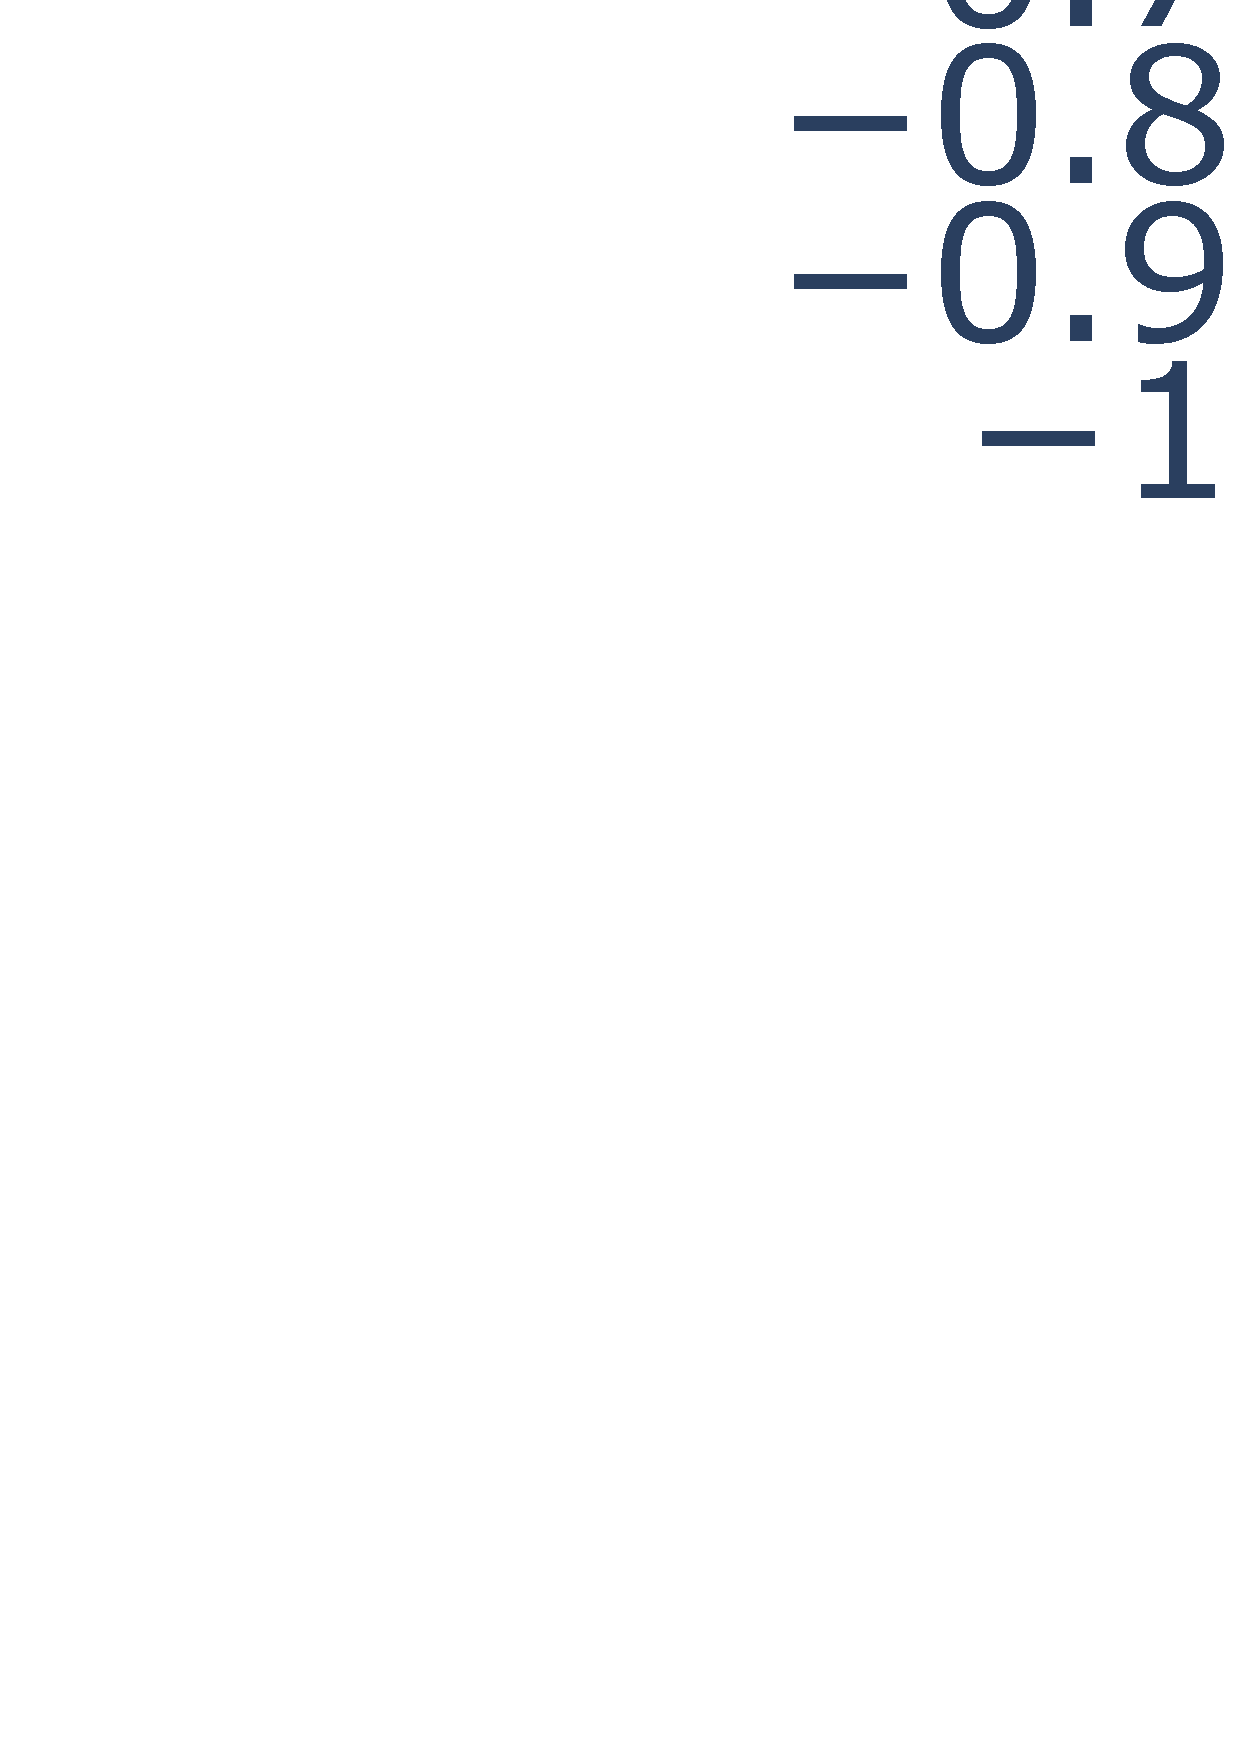
\includegraphics[width=0.8\linewidth]{images/01ContinuousVsDiscrete.pdf}
  %   \caption{Discrete samples (black points) from a continuous wave (grey line). Note that the amplitude is also truncated}
  %   \label{fig:ContinuousVsDiscrete}
  % \end{figure}
  
\section{Results}

\section{Discussion + Conclusion}

\section{References}
\printbibliography[heading=none]

\end{document}
